\documentclass{article}
\usepackage[a4paper, margin=2.5cm]{geometry} 
\usepackage[T1]{fontenc} %lädt Deutsche schriftzeichen
\usepackage{amssymb}%für Mathe
\usepackage{setspace} %für Zeilen Abstand 
\usepackage[none]{hyphenat} % Silbentrennung deaktivieren 
\usepackage{fancyhdr}%Kopf und Fußzeile: https://de.overleaf.com/learn/latex/Headers_and_footers
\usepackage{graphicx}%Zum Bilder einfügen
\usepackage{caption}%captions für bilder
\usepackage{float}%glaube auch für Bilder
\usepackage[dvipsnames]{xcolor}%Für Farbe 
\usepackage{colortbl}%farbe für tabelle
\usepackage{wrapfig}%Für gescheites einfügen von Bildern
\usepackage[ddmmyyyy]{datetime}%zum bearbeiten vom Datumgs Format
\renewcommand{\dateseparator}{.}%ändern von / zu .
\usepackage{url} % make urls clickable
\usepackage[scaled]{helvet}               %Default helevet schriftart
\renewcommand{\familydefault}{\sfdefault} %Default helevet schriftart
\usepackage{hyperref}%Hyperlinks
\usepackage{listings}%Code meines wissens nach
\usepackage{tcolorbox}%textboxen erweiterung
\usepackage{tocloft}%Abbildungsverzeichnis


\setlength{\parindent}{0pt}%Indent von zeilen weg

\fontsize{12}{13}

\title{Projekt Spieleentwicklung: Omega Sprinter}
\author{Nils Brück}
\date{\today}

\renewcommand{\contentsname}{Inhalsverzeichnis}%Umbenenen des Inhaltsverzeichnisses

\renewcommand{\listfigurename}{Abbildungsverzeichnis}

\renewcommand{\listtablename}{Listingsverzeichnis}


\captionsetup{justification=raggedright, singlelinecheck=false, font={scriptsize, it, color=gray}}%linksbündige, kleine, kursive, farbige caption

\begin{document}

\thispagestyle{empty}


\begin{Huge} 
	\textcolor{Black}{Projekt Spieleentwicklung: Omega Sprinter}
\end{Huge} \newline


\vspace{20cm}

\begin{tabular}{l l}
	
	Name: &Nils Brück\\
	
	\vspace{5mm}
	
	Datum: &\today\\
	
	\vspace{5mm}
	
	Klasse: &11BGx3\\
	
	Fach: &Praktische Informatik\\
	
	Fachlehrer:& Danilo Magdeburg\\
\end{tabular}

\newpage

\setcounter{page}{1} % Neustart der Seitenzählung

\pagenumbering{roman}%nummerstyle ändern

\pagestyle{fancy}
\fancyhf{}
\fancyhead[HL]{Nils Lasse Brück}
\fancyhead[HC]{Projekt Spieleentwicklung: Omega Sprinter}
\fancyhead[HR]{Praktische Informatik}
\fancyfoot[R]{\thepage}

\tableofcontents

\listoffigures

\listoftables

\newpage

\setcounter{page}{1} % Neustart der Seitenzählung

\pagenumbering{arabic}%nuberstyle ändern

\section{Einleitung}

Omega Sprinter ist ein 2D-Jump-and-Run Spiel mit Run-and-Gun Elementen. Das Spiel wurde im Rahmen des Schulunterrichts konzipiert und entwickelt. Voralge für dieses Projekt sind die klassischen Mega Man Spiele, also Platforming und lineares Leveldesign,sowie die Möglichkeit zu Schießen. \\
In der folgenden Dokumentation werden Spielidee, Entwurf, Durchführung und ein Fazit für das Projekt beschrieben. 

\section{Planung}

\subsection{Produkt und Idee in eigenen Worten}

Grundidee des Spiels ist ein 2D-Jump-and-Run, vereint mit Run-and-Gun-Elementen. Das grundlegende
Ziel ist es, das Levelende, ähnlich einer Flagge bei Super Mario, zu erreichen, um das Level abzuschließen.
Außerdem sollen vereinzelt Sammelelemente wie Münzen und Energiebälle zu finden sein. Der Schwerpunkt
des Spiels wird es sein, lineare Level mit Platforming-Einlagen und verschiedenen Gegnerarten abzuschließen
und nach Möglichkeit so viele Sammelobjekte wie möglich zu erhalten. Die HUD-Elemente sollen eher
sparsam sein: ein Energietracker als Lebensanzeige in Form einer Zahl von 1 bis 100 und ein Münzzähler,
der das gesamte Spiel hindurch hochzählt. In den Levels soll es Checkpoints geben, an denen ein Respawn
nach dem Tod möglich ist. Damit das Sterben auch bestraft wird, verliert der Spieler pro Tod Teile seiner
Münzen. Fallen diese auf Null, wird das Level beendet und der Spieler kommt zurück an den Levelanfang.
Um das Spiel zu beenden, muss das letzte Level erreicht und darin eine finale, schwere Herausforderung
bestehen. Grundlegend orientiert sich das Spiel an den originalen Mega Man Spielen.


\subsection{Prototypen}

Start und Idee in einem Level

\vspace{-2mm}

\begin{figure}[h]
	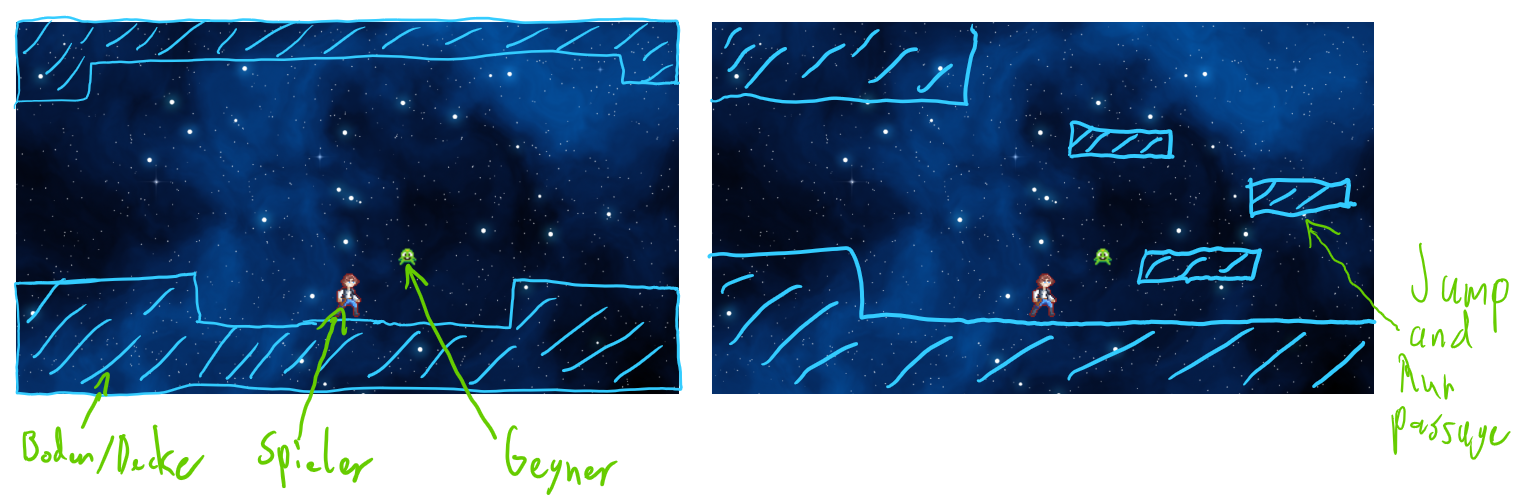
\includegraphics[scale=0.5] {Bilder/Start_game.png}
	
	\vspace{-2mm}
	
	\tiny{\caption {Prototyp Start/Ingame}}
	\label{Prototyp Start/Ingame}
\end{figure}

Schuss Mechanik

\vspace{-2mm}

\begin{figure}[h]
	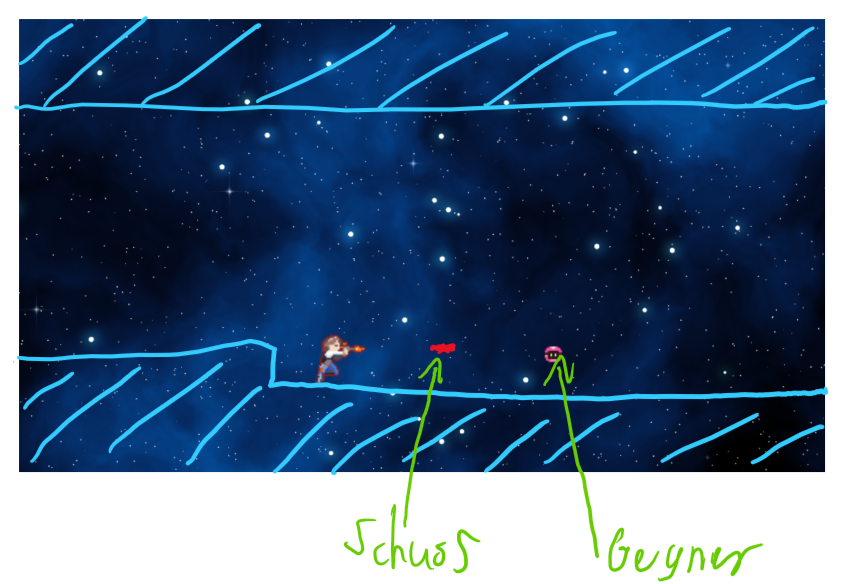
\includegraphics[scale=0.45] {Bilder/Game_shoot.png}
	
	\vspace{-3mm}
	
	\tiny{\caption {Schuss Mechanik}}
	\label{Schuss Mechanik Idee}
\end{figure}

\newpage

Ziel eines Levels

\vspace{-2mm}

\begin{figure}[h]
	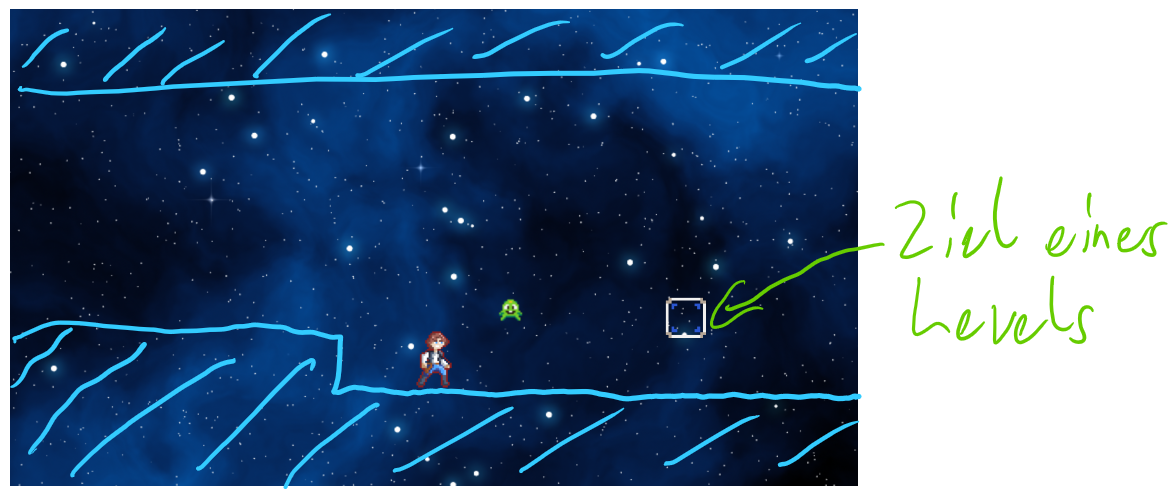
\includegraphics[scale=0.4] {Bilder/Goal_hah.png}
	
	\vspace{-2mm}
	
	\tiny{\caption {Levelziel}}
	\label{Levelziel Idee}
\end{figure}


\subsection{Versionierung \& Meilensteine}

Für die Versionierung wird Github und Git genutzt.\\
\newline
Meilensteine sind:
\begin{enumerate}
	\item {07.05.26 Erstes simples Jump and Run Level bauen}
	\item {14.05.26 Einfügen von Gegnern und Levelabschluss}
	\item {21.05.26 Einfügen von Schuss Mechanik auf X-Achse}
	\item {28.05.26 Erweitern um mehr Level \& Boss-Level}
	\item {Je nach Zeit erweitern der Schuss Mechanik auf Y-Achse}
\end{enumerate}

\section{Entwürfe}

Diese Sektion behandelt die Strukturgramm Entwürfe für die Grundlegendsten Mechaniken im Spiel.

\subsection{Entwurf Horizontales Movement des Spielers}

\vspace{-5mm}

\begin{figure}[h]
	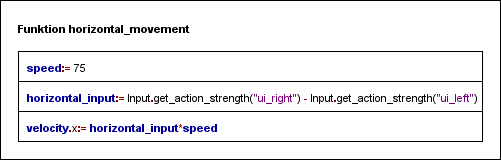
\includegraphics[scale=0.8] {Bilder/Funktion_horizontal_movement.png}
	
	\vspace{-3mm}
	
	\tiny{\caption {Strukturgramm Horizontales Movement}}
	\label{Struckturgramm horizontal}
\end{figure}

\newpage

\subsection{Entwurf: Input des Spielers}

\vspace{-5mm}

\begin{figure}[h]
	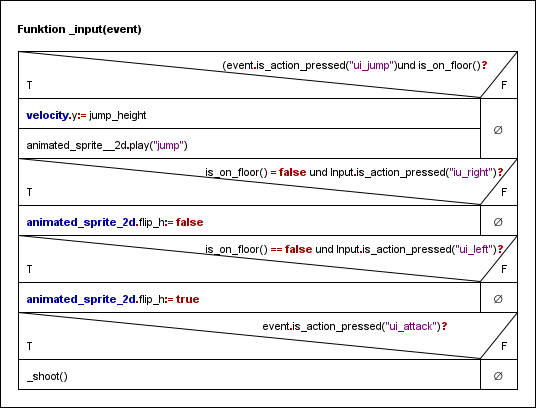
\includegraphics[scale=0.7] {Bilder/Funktion__input.png}
	
	\vspace{-3mm}
	
	\tiny{\caption {Strukturgramm User Inputs}}
	\label{Struckturgramm input}
\end{figure}

\subsection{Entwurf: Gegnerinteraktion}

\vspace{-5mm}

\begin{figure}[h]
	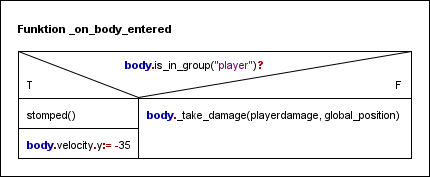
\includegraphics[scale=0.8] {Bilder/Funktion__on_body_entered.png}
	
	\vspace{-3mm}
	
	\tiny{\caption {Strukturgramm Gegnerinteraktion}}
	\label{Struckturgramm enemy_entered}
\end{figure}

\section{Durchführung}

In dieser Sektion der Dokumentation wird die aktive Durchführung des Projekts behandelt.

\subsection{Beschreiben des Ablaufs der Implementierung}

Zu beginn stand die Ideenfindung im Zentrum. Zum finden einer Idee haben Retro-Spiele als Beispiele im Mittelpunkt gestanden. Zuerst war die Spielidee am originalen Metroid orientiert. Nach weiterem suchen kam die klassischen Mega Man spiele auf, welche dann zur Hauptidee für das Projekt wurden. Damit waren dann Leveldesingidee und ungefähren HuD Elemente bestimmt.\\
Für die Implementierung wurde sich für beginn sehr stark an einem Online-Tutorial orientiert und Teilweise Claude Sonnet 4.6. In diesem wird das erstellen eines simplen Spielers mit Animationen, sowie das erstellen eines Tylemap-Layers. Als nächstes wurde mit dem selben Tutorial und anderen Online Tutorials eine Kamera hinzugefügt, welche dem Spieler durch das Level folgt. Als nächstes wurde ein Gegner in der Art eines klassischen Koopas aus Super Mario implementiert. Dieser dreht immer an einer Wand oder Abgrund um und läuft in die entgegengesetzte Richtung. Um dem Gegner noch Funktionalität zu bieten, wie das abziehen von Leben wurde noch eine HuD mit Gamestate Skript für Funktionalität von Leben und Coins hinzugefügt. Dafür wurde Hauptsächlich der schon geschriebene Code genutzt, sowie die offizielle Dokumentation von Godot. Auch wurde mit dem Gamestate die erste Funktionalität des Sterbens hinzugefügt. Nachdem die meisten Funktionalitäten für Spieler und Gegner fertig sind, beginnt der Level-bau. Durch den Bereit erstellten TyleMap-Layer war dies nicht schwierig zu Implementieren. jedoch musste noch das zuvor bereits erstellte Level-ziel eingepflegt werden. Das letzte zu implementierende Feature war ein Checkpoint im Level und das Verbinden mit den Coins und dem schon bereits existierenden Respawnpoint. Nach dieser Implementierung und dem Erweitern um einen Level Auswahl Screen als Main-Szene und einem Danke am Ende des Spiels war der Teil des Implementierens abgeschlossen. \\
Während des Programmierens und danach gab es verschiedenste Tests und Spieldurchläufe zum Finden von Bugs. Häufig gab es Problematiken mit kleiner Code abschnitten, aber auf Bugs und Fehlerbewältigung wird noch in einem späteren Abschnitt eingegangenen.\\

\subsection{Beschreibung des Spielablaufs, Screenshots und Codeausschnitte}

Zu beginn ist der Spieler in einem Level Auswahl Bildschirm in diesem kann dieser dann durch Springen in die ausgewählte Box zum Gewünschten Level gelangen. 

\begin{figure}[h]
	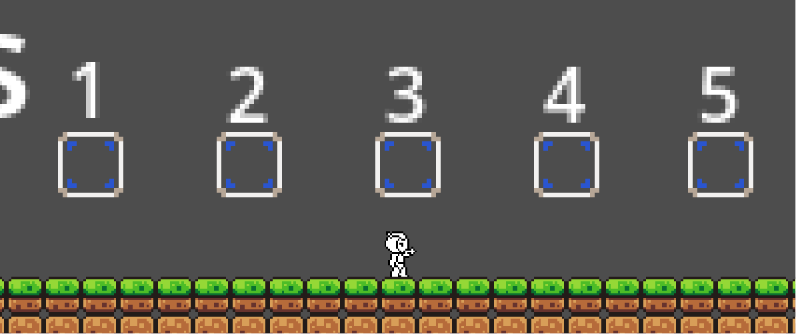
\includegraphics[scale=0.7] {Bilder/levelauswahl.png}
	
	\vspace{-3mm}
	
	\tiny{\caption {Levelauswahl Bildschirm}}
	\label{Levelauswahl Szene}
\end{figure}

\vspace{-3mm}

Nachdem der Spieler sein Level gewählt hat wird durch die Box in welcher dieser Springt die Szene des Levels geladen. Da diese Box auch für das Level-ende genutzt wird diese Interaktion vom levelende.gd Skript gehandhabt.

\vspace{-3mm}

\begin{table}[h]
\begin{tcolorbox}[colframe=Black, sharp corners, boxrule=0.5mm, colback=white]
	
	\vspace{-5mm}

\begin{lstlisting}[language=Python]
extends Area2D
	
#Ermoeglicht das aendern der Szene im Inspektor
@export var next_level: String = "res://level/level_2.tscn"
	
func _ready() -> void:
	
	#Erkennt wenn ein Node2D die Area betritt
	body_entered.connect(_on_body_entered)

func _on_body_entered(body: Node) -> void:
	#Checkt ob Player oder anderer Body Entered
	if body.is_in_group("player"):
		#Ruf die Szene aus next_level auf
		get_tree().call_deferred("change_scene_to_file", next_level)
\end{lstlisting}
\end{tcolorbox}
\vspace{-5mm}

\tiny{\caption {Level-ende}}
\label{Levelende.gd}
\end{table}

Im Level stehen dem Spieler die Grundlegenden Mechaniken des Laufen Springen und Schießens zur Verfügung.
Das Laufen, also das Bewegen auf der x-Achse, ist mit der Funktion horizontal\_movement() geregelt. In dieser Bekommt der Spieler eine Geschwindigkeit zugewiesen und die Richtung wird durch die Inputs des Spielers ermittelt. Aus dem Geschwindigkeitswert und der Richtung wird dann die Geschwindigkeit auf der x-Achse bestimmt. 

 \begin{table}[h]
 	\begin{tcolorbox}[colframe=Black, sharp corners, boxrule=0.5mm, colback=white]
 		
 		\vspace{-5mm}
 		
 \begin{lstlisting}[language=Python]
func horizontal_movement():
	var speed = 75
	# if keys are pressed it will return 1 for ui_right,
	# -1 for ui_left, and 0 for neither
	var horizontal_input = Input.get_action_strength("ui_right") 
		- Input.get_action_strength("ui_left")
	
	#Horizontale Geschwindigkeit bewegt Spieler nach links und rechts
	#Basiert auf User Input
	velocity.x = horizontal_input * speed
 \end{lstlisting}
 	\end{tcolorbox}
 	\vspace{-5mm}
 	
 	\tiny{\caption {Funktion Horizontales Movement}}
 	\label{Player horizontal_movement()}
 \end{table}

Um ein vollständiges Jump-and-Run erlebnis zu bieten wird noch eine Sprung Funktion benötigt, diese wird in der \_input Funktion geregelt. In dieser wird die im Player Skript festgelegte Sprunghöhe auf die Geschwindigkeit in y-Richtung angewendet.

\begin{table}[h]
	\begin{tcolorbox}[colframe=Black, sharp corners, boxrule=0.5mm, colback=white]
		
		\vspace{-5mm}
		
\begin{lstlisting}[language=Python]
#Checkt auf User Input und ob der Spieler auf dem Boden ist
if event.is_action_pressed("ui_jump") and is_on_floor():
	#Variable Sprunghoehe setzt die Geschwindigkeit in y-Richtung fest
	velocity.y = jump_height
	#Die Sprites des Spieler startet die Sprung animation
	animated_sprite_2d.play("jump")
\end{lstlisting}
	\end{tcolorbox}
	\vspace{-5mm}
	
	\tiny{\caption {Funktionsabschnitt Sprung}}
	\label{Player jump}
\end{table}

Level Eins ist sehr simpel gehalten und bietet kaum Schwierigkeit um den Spieler in das Spiel rein finden zu lassen. Auch sind direkt am Anfang Münzen platziert um dem Spieler direkt das Hauptsammelobjekt des Spieles zu Präsentieren. neben den Münzen ist auch eine Plattform in der Luft zu sehen, welche dem Spieler gleich mitteilt, dass es die Möglichkeit gibt Vertikales Movement zu nutzen. 

\begin{figure}[h]
	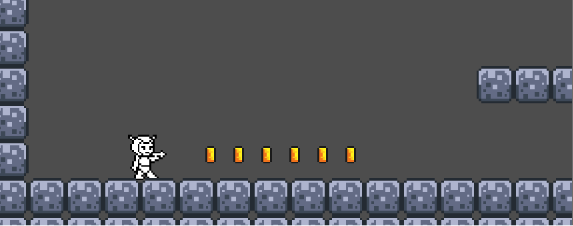
\includegraphics[scale=0.9] {Bilder/lev1start.png}
	
	\vspace{-3mm}
	
	\tiny{\caption {Level 1 Start}}
	\label{Level 1 start}
\end{figure}

\newpage

Schreitet der Spieler voran bekommt er einen Gegner zu sehen, sowie einen großen Schriftzug "Press E to Shoot". Damit macht man den Spieler auf die Schuss-Mechanik aufmerksam und zeig neben der Klassischen Jump-and-Run Methode des Heraufspringen noch eine weitere Methode um die Gegner zu besiegen.  

\begin{figure}[h]
	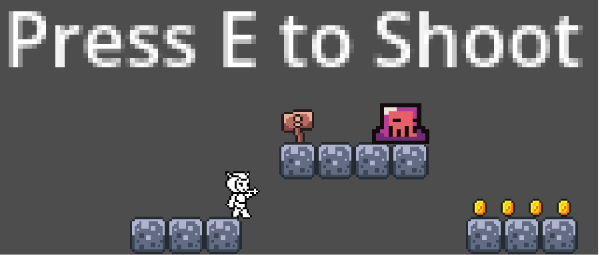
\includegraphics[scale=0.9] {Bilder/lev1erstergegner.png}
	
	\vspace{-3mm}
	
	\tiny{\caption {Level 1 Erster Gegner}}
	\label{Level 1 Enemy}
\end{figure}

Damit das Schießen überhaupt Funktioniert wird eine Schuss Funktion im Player benötigt und ein Skript für das Geschoss selber. \\
Als erstes kommt ins Player-Skript die \_shoot() Funktion. In dieser das Geschoss initialisiert und über einen Marker2D dessen Spawn-position bestimmt. Außerdem wird darüber noch ein offset und die direction bestimmt damit diese mit dem Spieler übereinstimmt. Als letztes wird die Szene als Childnode hinzugefügt und ein Cooldown aktiviert, damit man nicht durchgängig Schießen kann. 

\begin{table}[h]
	\begin{tcolorbox}[colframe=Black, sharp corners, boxrule=0.5mm, colback=white]
		
		\vspace{-5mm}
		
\begin{lstlisting}[language=Python]
func _shoot() -> void:
	#Checkt pb der Cooldown noch laeuft wenn ja
	#gibt es nichts zurrueck und bricht damit ab
	if shoot_cooldown > 0:
		return

	#Inizialisiert/Laedt die Bullet Szene vor
	var bullet = bullet_scene.instantiate()
	
	#Setzt die Bullet grundsaetzlich an die Marker2D Position
	var offset = muzzle.position
	#Nimmt sich den Absoluten offset also immer positiv
	#Multipliziert den offset mit -1 oder 1 fuer die richitge Richtung
	offset.x = abs(offset.x) * (-1 if animated_sprite_2d.flip_h else 1)
	#Kombiniert die Posioton der Bullet mit dem offset
	bullet.global_position = global_position + offset
	#Passt die ganze Bullet auf die Richtung an
	bullet.direction = -1 if animated_sprite_2d.flip_h else 1.0
	#Hohlt die Bullet in den Scene Tree als Child um sie abzuspielen
	get_tree().current_scene.add_child(bullet)

	#Setzt den Cooldwon neu
	shoot_cooldown = 0.3
\end{lstlisting}
	\end{tcolorbox}
	\vspace{-5mm}
	
	\tiny{\caption {Funktion Schuss des Players}}
	\label{Schuss Funktion Player}
\end{table}

\newpage

Das Geschoss selber benötigt auch noch ein Skript. Am wichtigsten sind die \_on\_body\_entered() und die \_on\_area\_entered() Funktionen, welche bestimmen ob das Geschoss mit einem anderen Körper oder einer anderen Area kollidiert. Besonders ist noch die Abfrage nach der Gruppe wichtig damit die Funktion nur auslöst wenn ein Gegner getroffen wird. 

\begin{table}[h]
	\begin{tcolorbox}[colframe=Black, sharp corners, boxrule=0.5mm, colback=white]
		
		\vspace{-5mm}
		
\begin{lstlisting}[language=Python]
func _on_body_entered(body: Node) -> void:
	#Beruehrt der Player soll nichts passieren
	if body.is_in_group("player"):
		return
	#beruehrt der Gegner wird die Funktion ausgefuert
	if body.is_in_group("enemies"):
		#Funktion des Gegners um ihn zu entfernen
		body.stomped()
		#Animation fuer das Geschoss und das verschwinden davon
		_explode()

func _on_area_entered(area: Area2D) -> void:
	#Hohlt sich die Uebergeordnete Node der Area
	var parent = area.get_parent()
	#Ueberprueft ob Gegner
	if parent.is_in_group("enemies"):
		#Funktion um gegner zu entfernen wird gecallt
		parent.stomped()
		#Animation fuer das Geschoss und das verschwinden davon
		_explode()
\end{lstlisting}
	\end{tcolorbox}
	\vspace{-5mm}
	
	\tiny{\caption {Funktion Schuss des Geschosses}}
	\label{Schuss Funktion Bullet}
\end{table}

Das ganze sieht dann Ingame so aus:

\begin{figure}[h]
	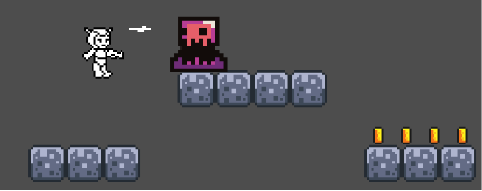
\includegraphics[scale=0.7] {Bilder/lev1shootgegner.png}
	
	\vspace{-3mm}
	
	\tiny{\caption {Level 1 Gegner Abschießen}}
	\label{Level 1 Shoot}
\end{figure}


Und wenn das Geschoss dann Getroffen hat und der Gegner verschwindet. 



\begin{figure}[h]
	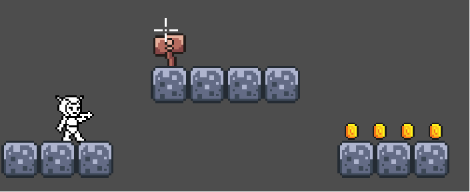
\includegraphics[scale=0.7] {Bilder/lev1totgegner.png}
	
	\vspace{-3mm}
	
	\tiny{\caption {Level 1 Gegner Getroffen und Entfernt}}
	\label{Level 1 gegner death}
\end{figure}

\newpage

Schreitet man im Level voran und schließt die erste Passage ab trifft man auf einen Liveball, welcher die Leben des Spielers regeneriert. Falls der Spieler bis dahin bereits Leben verloren, wird der Liveball beim Einsammeln aktiviert und regeneriert 15 Leben. Hat der Spieler mehr als 85 Leben, so wird auf maximal 100 Leben regeneriert.\\
Um dies zu realisieren wird ein Gamestate genutzt, welcher die Variablen handhabt, welche von verschiedensten Skripten gebraucht wird. Daneben gibt es noch das Liveball Skript in dem nur die Animationen und die Kollision geregelt werden, deswegen wird auch auf ein Codebeispiel davon verzichtet.\\

\vspace{-3mm}

\begin{figure}[h]
	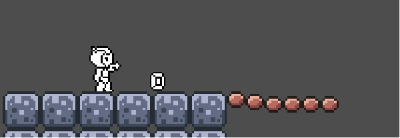
\includegraphics[scale=0.9] {Bilder/lev1liveball.png}
	
	\vspace{-3mm}
	
	\tiny{\caption {Level 1 Liveball}}
	\label{Level 1 Liveball}
\end{figure}

Wenn das Level abgeschlossen ist kann man mit den bereits erläuterten Levelenden zum nächsten Level gehen.

\begin{figure}[h]
	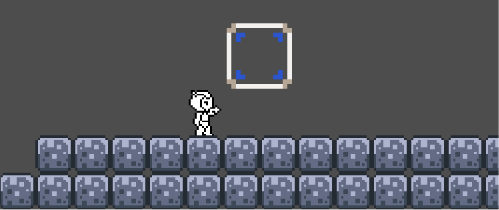
\includegraphics[scale=0.7] {Bilder/lev1ende.png}
	
	\vspace{-3mm}
	
	\tiny{\caption {Level 1 Levelende}}
	\label{Level 1 ende}
\end{figure}

Im zweiten Level gibt es erst zur Mitte ein neues erwähnenswertes Element. in der Mitte dann kommt ein Checkpoint zum Einsatz, damit der Spieler bei einem Tod nicht das ganze Level neu spielen muss. Besinderheit, am Checkpoint ist, dass wenn die Münzen auf Null Fallen wird dieser nicht mehr genutzt und der Spieler respawnt am Levelanfang. 


\end{document}